%!TEX root = ../main.tex

\section{Kruskal's Algorithm}


Kruskal's algorithm finds a minimum weight spanning tree in a 
connected, weighted, undirected graph. 

\begin{itemize}
    \item Step 1: Sort and renumber the edges in increasing
order of weight as $e_1, ..., e_n$. 
    \item Step 2: Create a graph $G$ with the same vertices as the
    original
    graph.
    \item Step 3: For each edge $e_i = (u, v)$, add the edge
    to the graph if and only if $u$ and $v$ lie in different
    components. To do this, we need two routines.
    \begin{itemize}
        \item Find: return the component for a vertex $u$.
        \item Union: merge two components together.
    \end{itemize}
    We are going to define a \href{https://en.wikipedia.org/wiki/Disjoint-set_data_structure}{union-find} data structure to
    solve this, which we will initialize to $n$ singleton components.
\end{itemize}

\subsubsection{Union-Find}

Let's look at various attempts to implement this data structure.

\begin{enumerate}
    \item First attempt. Keep an array where the index $i$ tells you
    what
    component $v_i$ is in. Initially, each vertex belongs to its
    component, so the array is $A = [1, 2, 3, ..., n]$. We immediately
    notice that we can perform the find operation in
    $O(1)$ (just index into the array). What about union of $u$ and
    $v$? This takes $O(n)$ (you might need to reassign $n - 1$
    components). Using this approach, in
    the course of Kruskal's algorithm we will perform $n - 1$ unions 
    (we start from $n$ components and get to 1 component). Each takes
    order $n$, so we'll get overall $O(n^2)$. We want to do better.
    \item Second attempt. 
    Notice that when we perform union($u, v$), $u$'s set contains
    $n_1$ elements and $v$'s set contains $n_2$ elements. To do less
    operations, we ideally want to change the components of the set
    that is smaller. This operation still takes in the worst case $O
    (n)$. In this attempt, in addition to the array, we maintain a
    linked list for each set containing the elements in that set 
    (think of it as a reverse indexing from the component to the
    elements). An
    individual union operation could still take $\Theta(n)$ steps.
    However, any $k$ union operations performed by Kruskal take only
    $O(k\log(n))$ steps. We've moved from analyzing one operation to
    analyzing a sequence of operations (amortized analysis, we'll
    talk about this in a minute). Indeed, suppose you take the union
    of $A$ and $B$, where $|A| > |B|$. The cost of the operation is
    equal to the size of $B$. Set up a counter for each element in
    the data structure, and charge 1 to each element in $B$ for a
    union operation. How many times does an element get charged? Every
    time an element is charged, it joins a set that is as twice as
    large. Therefore, we can charge at most $\log(n)$ times, so the
    total cost of all $n - 1$ unions is $n\log(n)$. More careful
    analysis will show you that $k$ unions cost at most $k\log(k)$.
    This is an example of amortized analysis.
    \item Third attempt. The idea is to maintain each connected
    component as a tree (see Figure~\ref{fig:kruskal}). How long does
    the find operation
    take? Say
    the name of the component is the element at the root of the tree.
    For each node in the tree, keep a pointer to its parent.
    Finally, traverse up the tree until you find the root and you will
    have found the component. The cost is proportional to the height
    of each tree (note that all tree heights at all
    times are $O(\log(n))$, so this is what it costs to do a find). 
    To do a union operation, have one root point to the
    other root. We can do the same amortized trick we performed above,
    and we can make the root of the tree with fewer elements point up
    to the root of the other tree. Unions of arbitrary pairs of
    elements is also $O(\log(n))$. We've established that Kruskal
    performs $n - 1$ unions, but how many finds does it perform? It
    does $O(m)$ finds. Therefore, performing all the union-finds takes
    $O(m\log(n))$.
\end{enumerate}

\begin{figure}[hpt]
    \centering
    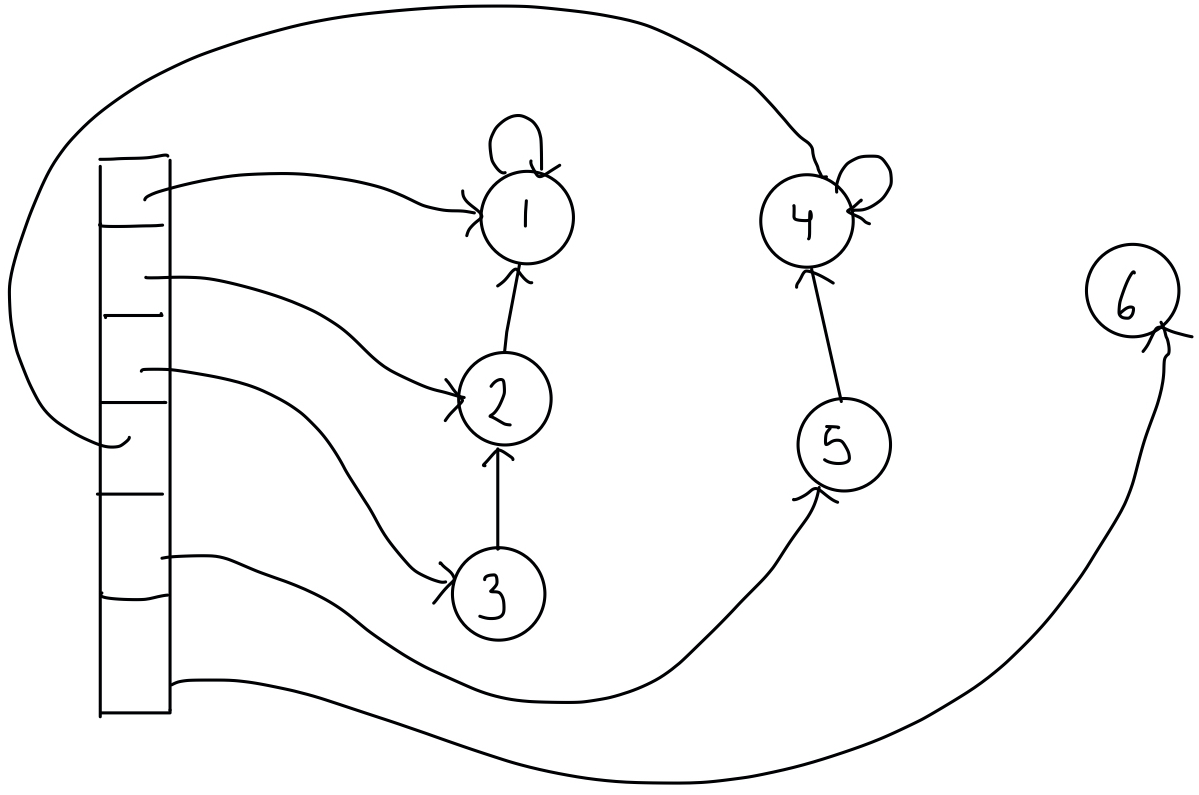
\includegraphics[width=0.65\textwidth]{figures/kruskal.jpeg}
    \caption{Data structure used for the third attempt}
    \label{fig:kruskal}
\end{figure}

The time complexity for Kruskal is $O(m\log(n))$. Indeed, we have to
first sort the edges by weights, so the union-finds are not in fact
the bottleneck. One optimization in the third attempt is called path
compression. The idea is that when you perform find($u$), for each
vertex encountered from the path from $u$ to the root, make it a child
of the root. 

Any sequence of $m$ operations starting from the initial
union find data structure on $n$ elements takes at most $O(m\log^*
(n))$ time, where $\log^*(x)$ is the number of times you need to take
the log of $x$ to make the value less than or equal to 1. For
instance,
$\log^*(16) = 3$, since you need to do $16 \to 4 \to 2 \to 1$.
The fact is $\log^*(n)$ is a \textbf{really} slow growing
function, so we can take interpret it as a constant. For example,
$\log^*(2^{16} = 65,536) = 4$, and $\log^*(2^{65,536}) = 5$. This is
more than the number of particles in the universe, so there's no way
that you will get a problem with an input bigger than this. Therefore,
we can treat it as almost constant.

\section{Prim's Algorithm}

In Prim's algorithm, we keep a set $S$, which we call the source side,
and we consider $V - S$, the remaining vertices that are not in $S$.
At every step we take the cheapest edge joining $S$ and
$V - S$. For each $v \in V - S$, maintain $d(v)$, which is the
weight of the cheapest edge from $v$ to some vertex in $S$. 

Initially, $S = \{ s \}$, and for every $v \in V - S$, we have that
$d(v) = w(s, v)$ if $(s, v)$ is an edge and $\infty$ otherwise. At
each iteration (see Figure~\ref{fig:prim}), when we move the vertex
$y$ that has the cheapest edge to a vertex in $S$, we need to update
every neighbor $v$ of $y$ so that $d(v) = \min(d(v), w(v, y))$.

\begin{figure}[hpt]
    \centering
    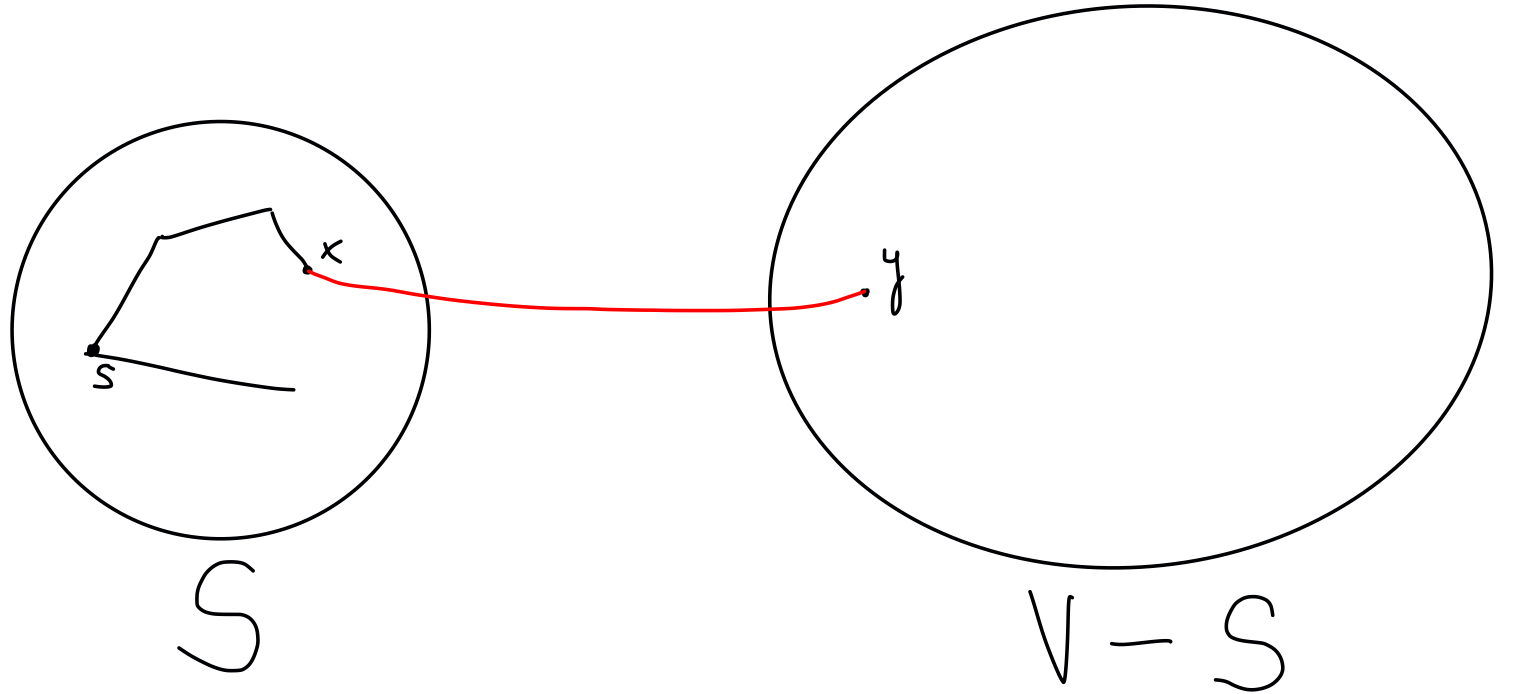
\includegraphics[width=0.65\textwidth]{figures/prim.jpeg}
    \caption{Prim's algorithm visualization}
    \label{fig:prim}
\end{figure}

\subsubsection{Time Complexity}

If we maintain the $d(v)$s in an array $A$, the complexity is $O(n^2)$
because we need to first find the minimum in $A$, and once we've found
the minimum we need to update all the neighbors of the minimum.

If we maintain the $d(v)$s in a min-heap, the complexity is $O(m\log
(n))$.

\section{Shortest Paths}

Let $G = (V, E)$ be a directed, weighted graph with a weight function
$w : E \to \mathbb{R}$. We assume $G$ is directed because we can
easily convert undirected shortest paths to directed shortest paths.

One common variation for this problem is the single source shortest
path. The problem is to find the shortest path from a given vertex $s$
to all the other vertices. Another variant is all-paths shortest path,
in which we need to find the shortest path from any $u$ to any
$v$.

\subsection{Single Source Shortest Path}

We will assume all edge weights are non negative, and we will solve
this using Dijkstra's Algorithm. The idea is to maintain a quantity $d
(v)$ for each vertex $v$ which is an upper bound on the length of the
shortest path from $s$ to $v$.










